\section{Methodology}
\label{sec:7_3_data}
In this section I briefly recall data collection pipeline and the simulation scenario adopted in this chapter, which basically replicates what I described in chapter \ref{chap:6_4cities}.

\subsection{The dataset}
The dataset I use for the following analyses is collected through the software described in chapter \ref{chap:2_dataset}. The subset sampling is the same performed in section \ref{sec:6_2_data}. Figure \ref{fig:7_3_ECDFs} recalls the main features of collected trips. In particular, in Turin, the 95\% of rentals covers less than 10 km and the 95\% of parking lasts less than 12 hours. 

\begin{figure}[th]
	\centering
	\subfloat[][CDF of travelled distances. X-axis is logarithmic.]
	{
		\label{fig:7_3_cdf_distance}
		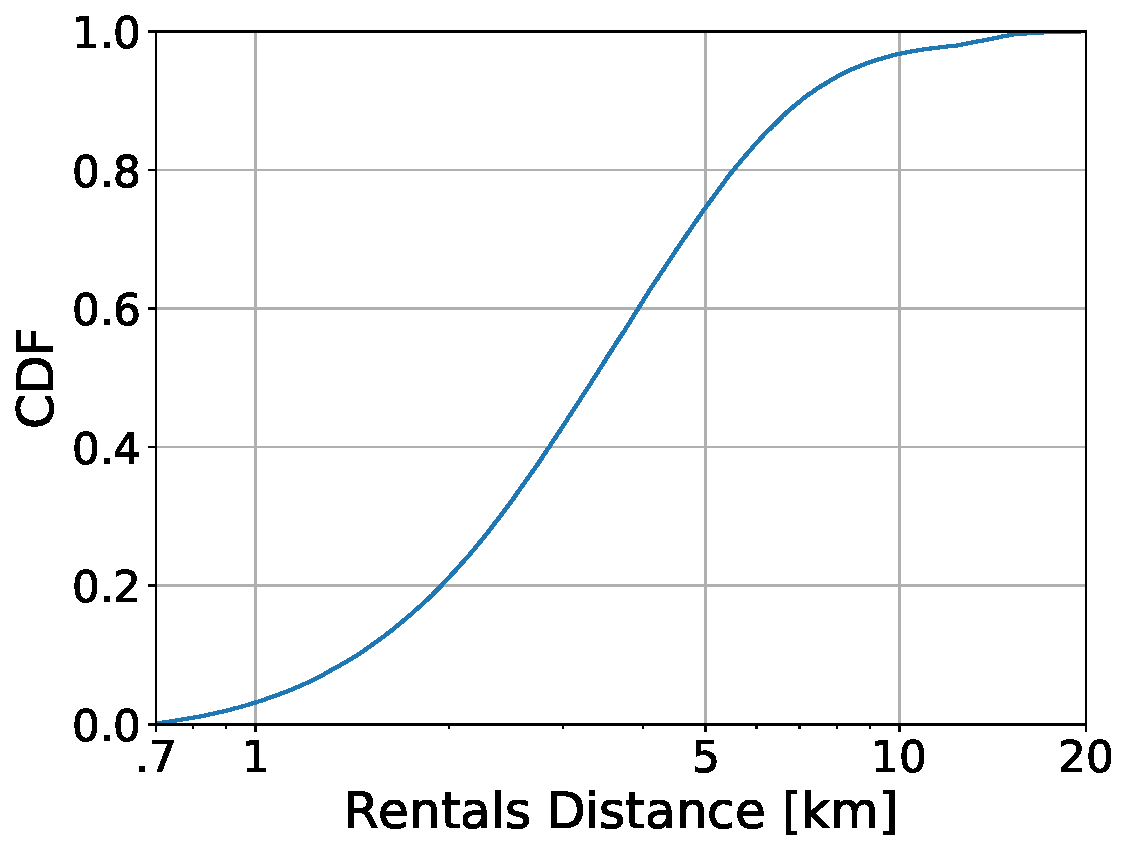
\includegraphics[width=0.45\columnwidth]{figures/CDF_distance.pdf}
	}
	\subfloat[][CDF of parking durations. X-axis is logarithmic, and limited to 2 days.]
	{
		\label{fig:7_3_cdf_duration}
		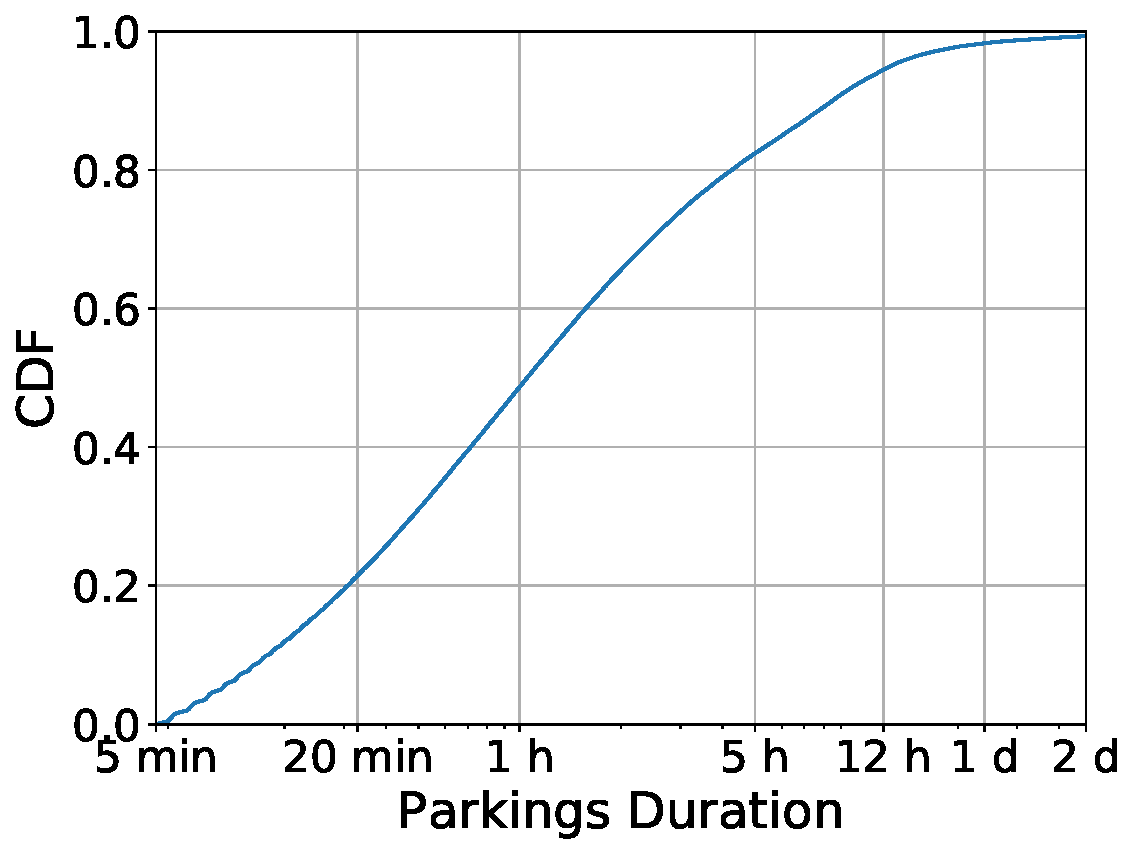
\includegraphics[width=0.45\columnwidth]{figures/CDF_duration.pdf}
	}
	\caption{Characteristics of the trips in our data-set.}
	\label{fig:7_3_ECDFs}
\end{figure}

\mc{introdurre qui gli spatial patterns}

\begin{figure}[th]
    \centering     %%% not \center
        \subfloat[][Number of Parkings.]
            {
            \label{fig:7_3_hm_max-parking}
            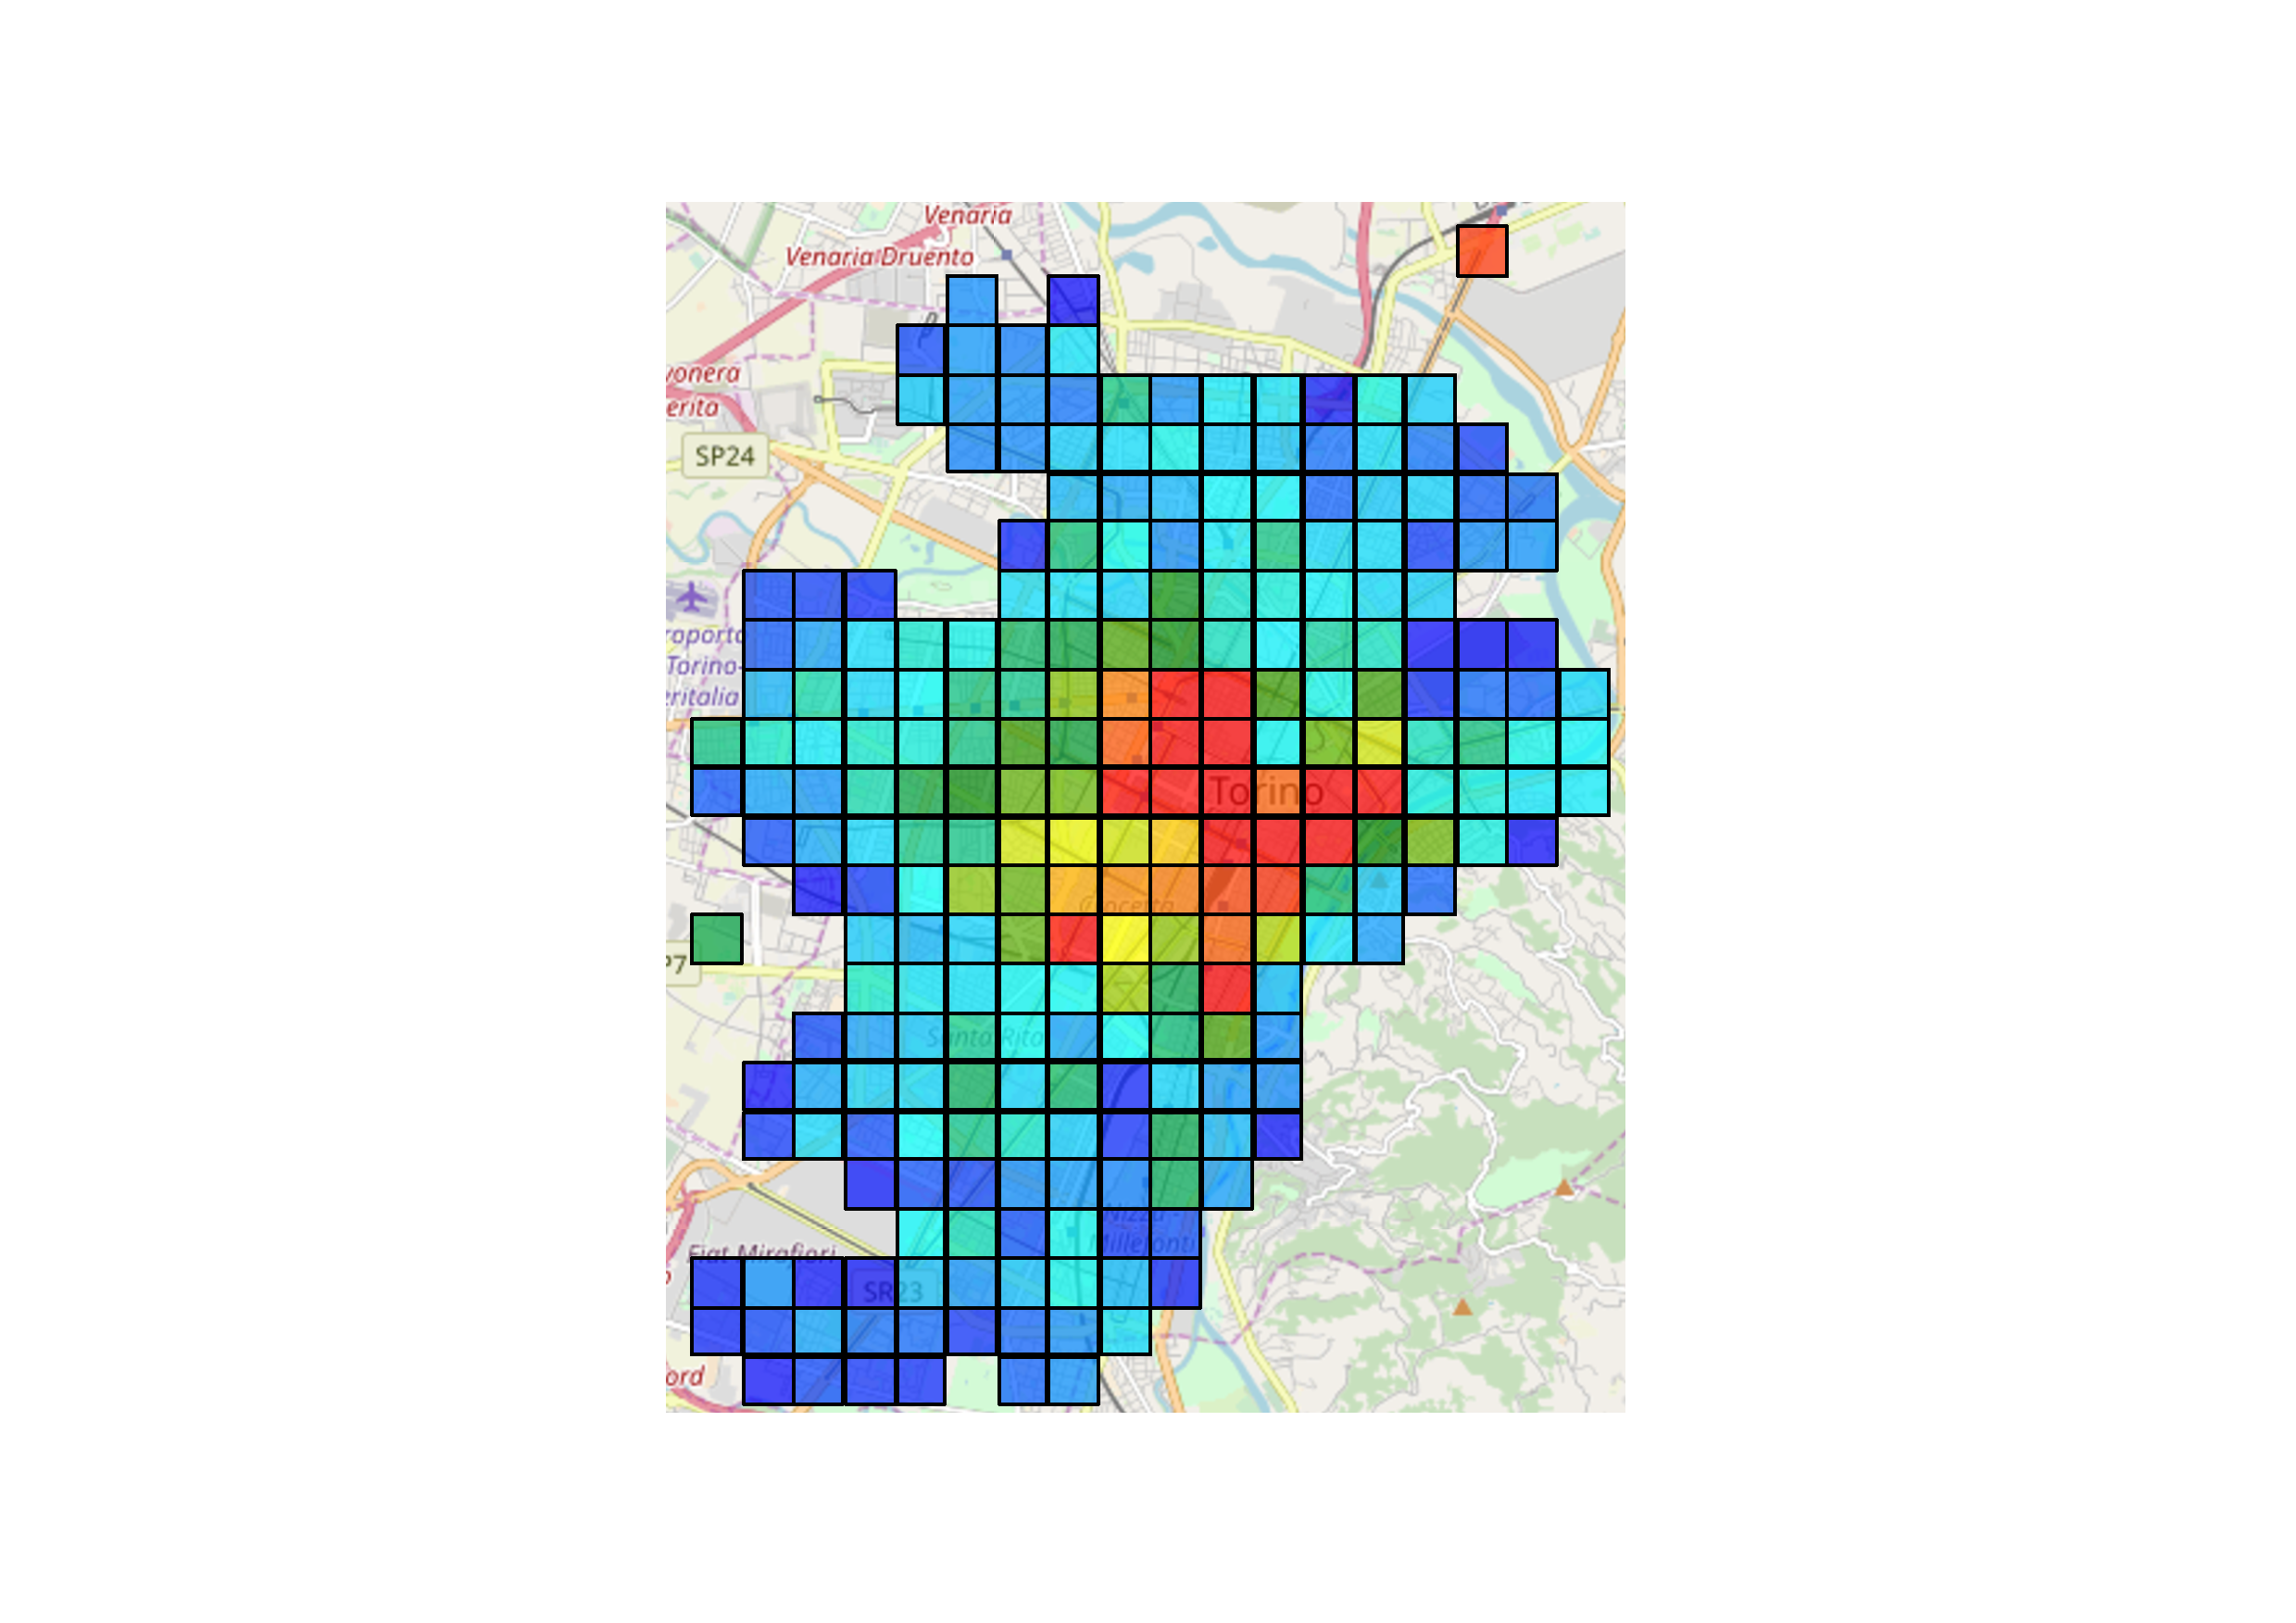
\includegraphics[width=0.35\columnwidth]{figures/Torino_NParkings.pdf}
            }
        \subfloat[][Average Parking Time.]
            {
            \label{fig:7_3_hm_avg-time}
            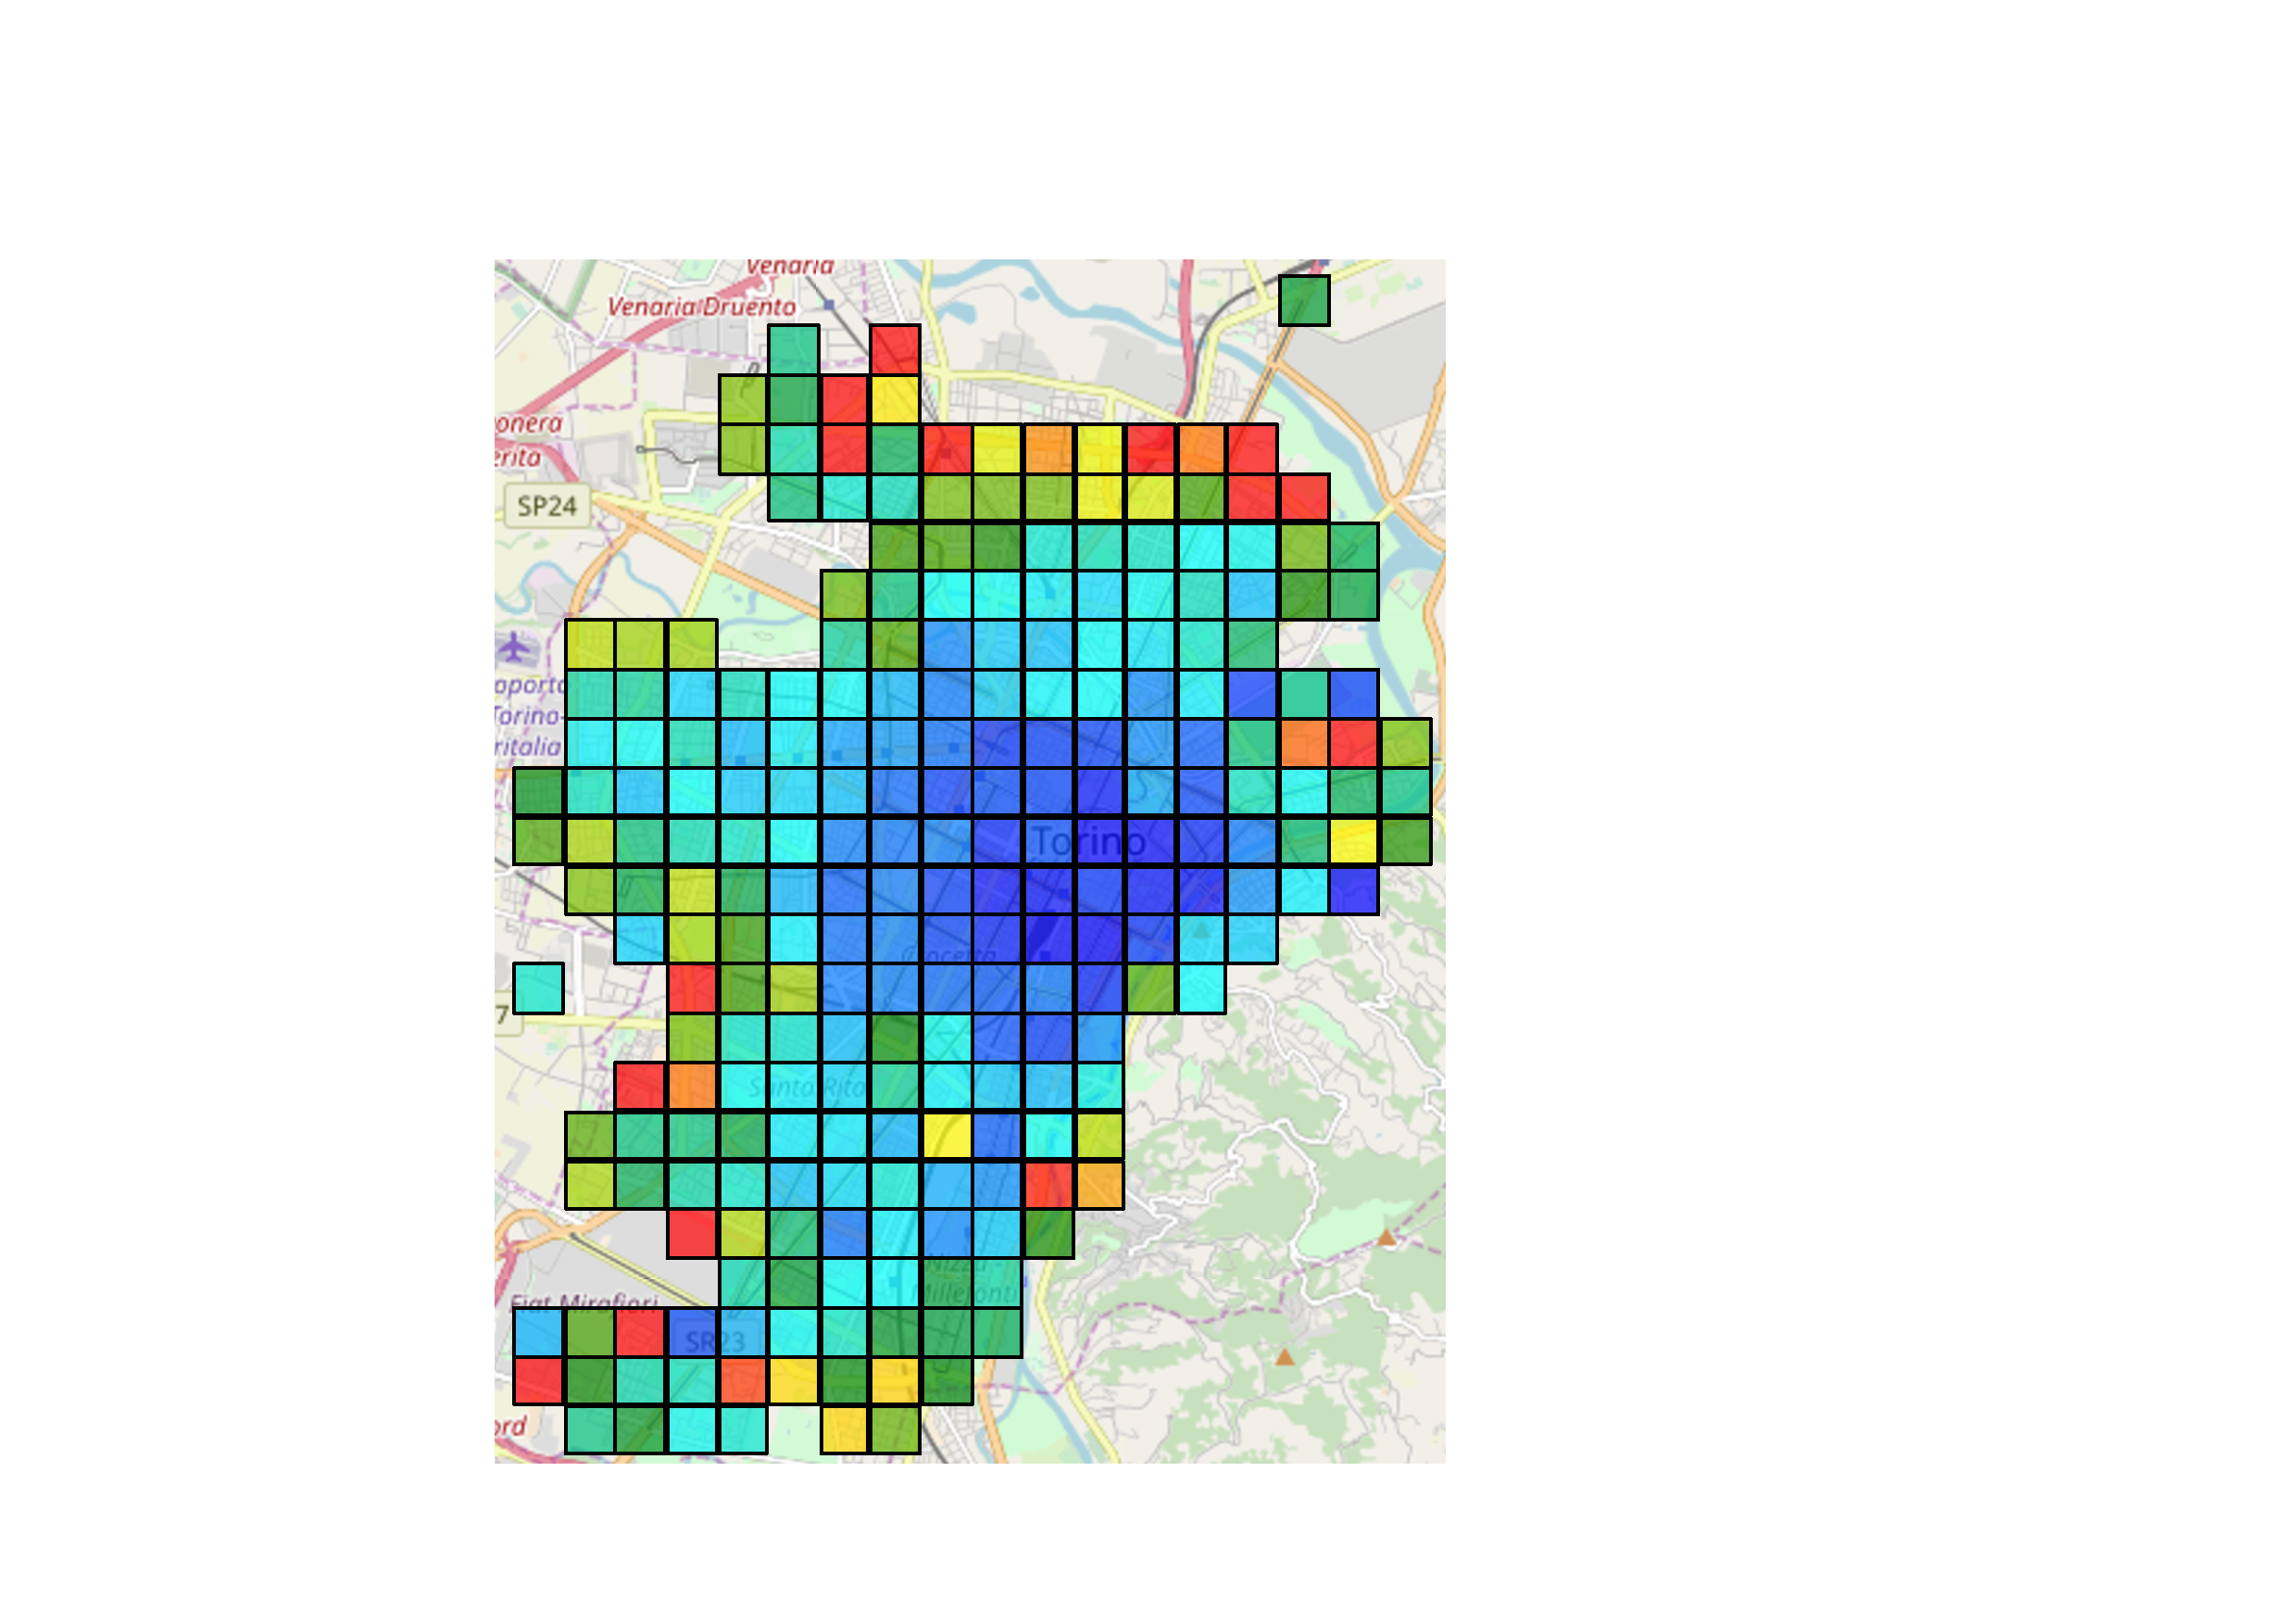
\includegraphics[width=0.35\columnwidth]{figures/Torino_AvgTime.pdf}
            }
    	\caption{Heatmaps showing (a) number of parkings per zone  and (b) average parking time per zone. Warmer areas have larger values. }
    	\label{fig:7_3_data_car}
\end{figure}

Figure \ref{fig:7_3_hm_max-parking} shows the heatmap of the total number of parkings in each city zone. The warmer the colour is, the more frequently cars are parked here. The hot areas correspond to the city centre which exhibits the highest number of parkings. Customers rely on car sharing for travelling and moving downtown, a working area full of shops and restaurants. The zones with more parkings are close to the train stations, where 47 parking events per day are observed on average.

Figure \ref{fig:7_3_hm_avg-time} shows the heatmap of the average parking time for each zone. Peaks are on borders of the operative area, where parking events last more than 24 hours. Few cars reach these peripheries  and rest unused for long time (see also rightmost part of Fig. \ref{fig:7_3_cdf_duration}). The lower values are registered in the downtown, where cars stay parked only for 85 minutes on average.

%On the contrary, few parkings are observed in the suburbs (down to less than 1 event per day), where people likely return home in the evening~\cite{UMAP}. 

%\section{Data collection and characterisation}
%\label{sec:7_3_data}
%
%Obtaining mobility data is fundamental in the design of transport systems. Nowadays, the diffusion of ICT technologies makes collecting actual usage data much simpler. Here, we present our approach to collect data from currently running FFCSs. For this, we designed and engineered \tool~\cite{UMAP}. It is composed by three modules: a data acquisition, a data normalisation and integration, and a data characterisation and analysis module. \tool is freely accessible as open source at~\cite{MicheleGithub}.
%
%\subsection{Data Acquisition}
%
%The first step consists in the data acquisition from the FFCS platform of interest. Each platform exposes information through a web-service that lets customers find positions of cars when available for rental. 
%\tool implements crawler-modules that harvests these web-service to collect, at periodic time instant, which cars are available. For now, we have developed crawlers for two FFCS providers, Car2Go and Enjoy, both offering services in Italy. For Car2Go,  we rely on their public APIs~\footnote{Car2Go API, \url{https://www.car2go.com/api/tou.htm}, service subject to approval by Car2Go. Approval granted in September 2016, service disconnected in January 2018.}, while for Enjoy we implemented a custom crawler by reverse engineering API. In both cases, the system returns the currently available cars using a JSON document, for each city in which they are present.
%\tool takes periodic \textit{snapshots} describing which cars are parked and ready for rental.
%
%In a nutshell, a car is described as an object annotated by information like plate, vehicle identification number (VIN), fuel level, model, parked location, etc. 
%This is instrumental for the customers, e.g., to choose which car to rent.
%This object is only present if the car is available, i.e., it is parked and free for a rental. When a customer reserves and rents it, the object disappears, and reappears later when the customer ends the rental, likely in a different location.
%
%\tool takes a snapshot $S(t)$ every minute, a reasonable time resolution to capture car rental and return events, while avoiding overloading the servers.
%In particular, we extract 
%the \textit{VIN} or \textit{plate} field to uniquely identify a car, the parking \textit{coordinates} reported with \textit{longitude} and \textit{latitude} by the in-car GPS, and the \textit{fuel} level of the car.\footnote{The GPS coordinates are only available if a car is parked and available. There is no risk for users' privacy during rentals. In addition no user's identifier is exposed. Therefore data is totally anonymized as there is no means to know who booked a car.}
%
%We started collecting data with \tool in December 2016, and we have collected more than a year of data in all the 22 and 5 cities where Car2Go and Enjoy offer service, respectively. 
%
%\subsection{Data Normalisation and Integration}
%
%In this second module we process and consolidate each snapshot $S(t)$ to obtain \textit{booking} and \textit{parking} periods for each car. The intuition is to track the availability of each car, and rebuild the history of parking and booking periods over time: when some customer books a car at time $[t-1,t)$, the latter ``disappears'' from the system starting from $S(t)$. We identify this events, and record it by creating a new booking, and setting the start time ($t_s=t$) and the start position. When the customer ends the booking, the car ``reappears'' in the system in $S(t2), t2>t$. We record this event, by setting the end time ($t_e=t2$) and end position of the booking. After that, for the same car, a new parking period starts, hence we record a new parking event with its initial time ($t_s=t2$) and its position. When the car ``disappears'' again in $S(t3),t3>t2$, we record end time ($t_e=t3$) of the parking event, and we start recording a new booking.
% 
%Next, we define a procedure to filter bookings and to obtain actual \textit{rentals}. The FFCS allows customers to reserve a car prior the actual rental starts. In case the customer cancels the reservation, the car becomes available, creating a booking in our data-set, for which no rental actually ever happened. Conversely, some bookings last for several days or weeks, e.g., due to a car going offline, or under repair. At last, the back-end system may sometimes fail, generating spurious bookings. \tool filters these artefacts to obtain actual {rentals}: Initial  and final positions must be at least 500\,m far apart, booking duration must be greater than 3 minutes, and shorter than 1 hour. %After filtering, our Turin dataset contains about 125\,000 actual rentals.
%
%At last, we need to estimate the possible driving path and length from the knowledge of only the initial and final position. Euclidean distance between starting and ending coordinates of the trip represents a lower bound of the real driven distance, since cars have to follow the topology of the city and traffic laws. To estimate the real driving distance, we apply a corrective factor, that we obtain again from data. In more details, given a rental, we use the information returned by the Google Directions API related to the best driving path from the  initial to the final position of the rental.~\footnote{\url{https://developers.google.com/maps/documentation/distance-matrix/}, freely available for a limited number of queries.} Then, we compute the ratio between the returned driving distance, and the euclidean distance. \reviewed{We collect this information at time the trip end is observed.}\footnote{Google Directions API factor eventual traffic congestion at different time of the day. As such, we include its impact in our model.}
%We repeat this for about 10\,000 trips, observing the distribution of the ratio which ranges between 1 and 2, with most of values around the median value of 1.4. We use the latter value as corrective factor to obtain the driving distance from the euclidean distance.
%
%In this work, \reviewed{we consider 8 weeks between September and  November 2017 for the Car2Go provider to optimise the charging station placement. We collected about 190\,000 bookings that generated 125\,000 actual rentals from the 377 cars of the Car2Go fleet in Turin. To verify the robustness of the solution, we use other two traces collected in June-July 2017 and December 2017-January 2018}.
%
%\reviewed{Our data takes into account all the rentals, also in presence of special events generating a higher demand (like strikes, sport events, concerts, etc.). Therefore our data captures both normal daily traffic patterns, and anomalies.}
%
%In the following, we provide a quick characterisation of the data, which is instrumental to guide the design of the charging station placement algorithms.
%
%\subsection{Data characterisation}
%
%First focus on the characterisation of the (estimated) distance travelled during rentals. This figure is interesting since it is directly related to the minimum amount of charge an electric car shall have to complete a trip.
%Fig. \ref{fig:cdf_distance} shows the empirical Cumulative Density Function (CDF) of the distances covered over all rentals. 97\% of the trips covers less than 10~km, roughly corresponding to the operative area diameter in Turin. The remaining 3\% are trips to and from the airport, up to 19 km far away.\footnote{The Turin airport has a reserved parking for Car2Go vehicles. It is about 15 km far away from the city centre. Distances for trips to the airport, reached by a straight highway, are not corrected.}
%
%Next, we investigate the parking duration. This figure is interesting since it is related to the amount of charge a parked car obtains when attached to a charging station.
%Fig. \ref{fig:cdf_duration} illustrates the empirical CDF of parking duration. Interestingly, more than half of the parking events lasts less than 1 hour. This is due to the high utilisation of cars in FFCS, especially during business hours.
%Conversely, 10\% of the parking events lasts more than 8 hours, with some cars that are left parked for days. The former are probably due to overnight parkings, while the latter hint for some cars parked in areas with few customers.
%
%\begin{figure}[th]
%    \centering
%        \subfloat[][CDF of travelled distances. X-axis is logarithmic.]
%        {
%            \label{fig:cdf_distance}
%            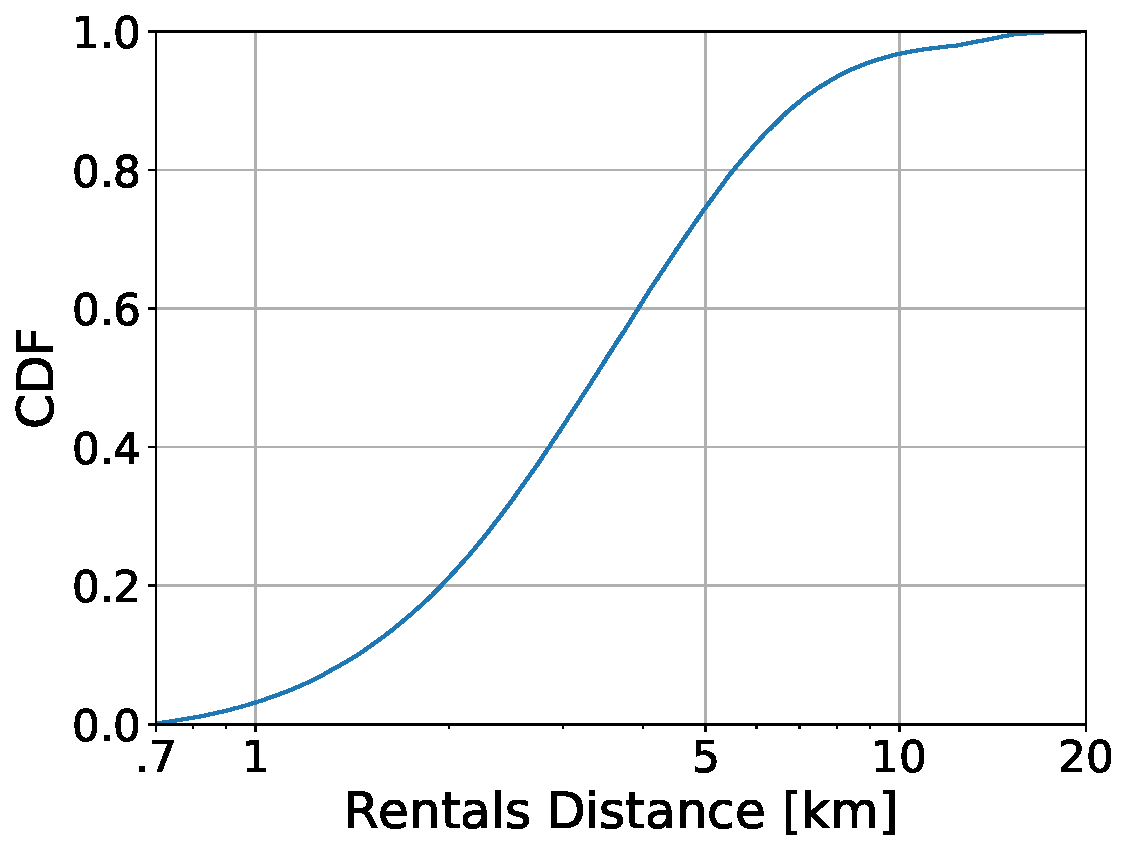
\includegraphics[width=0.45\columnwidth]{figures/CDF_distance.pdf}
%        }
%        \subfloat[][CDF of parking durations. X-axis is logarithmic, and limited to 2 days.]
%        {
%            \label{fig:cdf_duration}
%            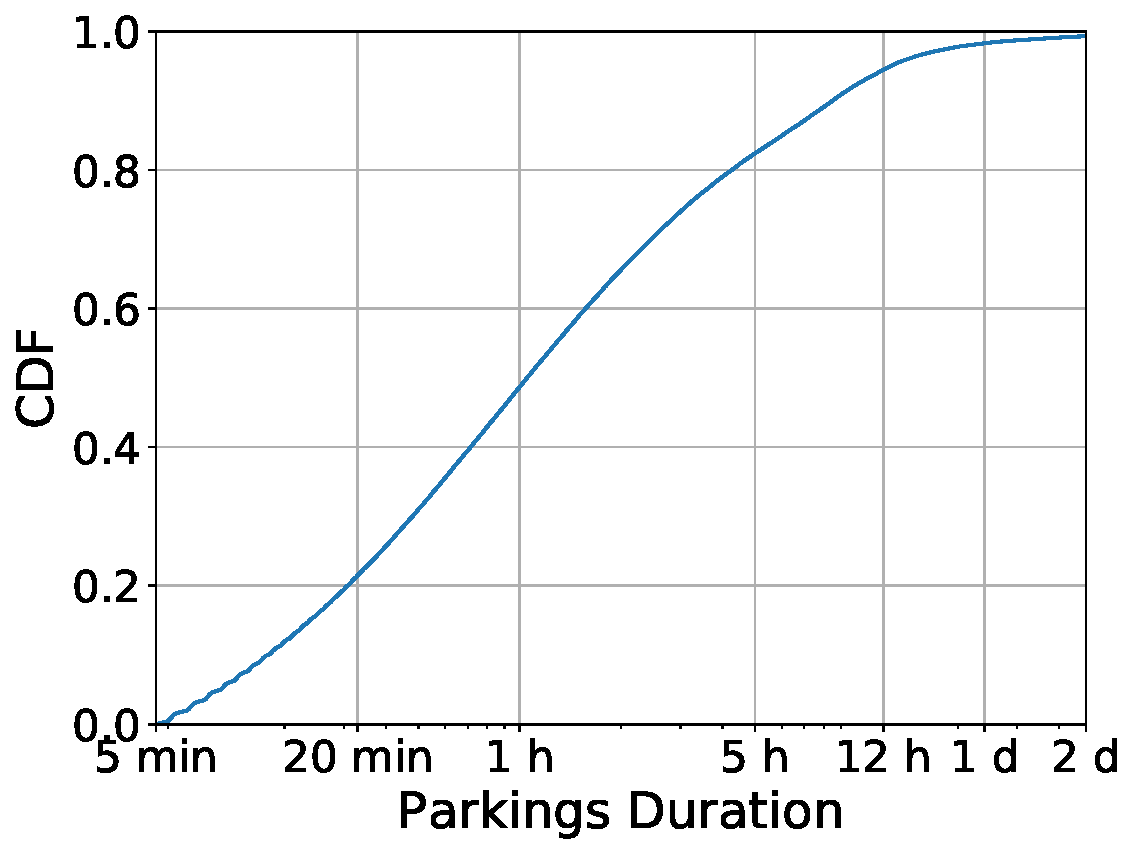
\includegraphics[width=0.45\columnwidth]{figures/CDF_duration.pdf}
%        }
%        \caption{Characteristics of the trips in our data-set.}
%        \label{}
%\end{figure}
%
%
%Next, we analyse how parking habits are different in the city area. For this, we divide the service operative area using a grid of squared zones of 500x500 meters, obtaining 261 zones covering Turin.
%For each zone, we compute the total number of parkings recorded and the average parking time.
%
%
%Fig. \ref{fig:hm_max-parking} shows the heatmap of the total number of parkings in each city zone. The warmer the colour is, the more frequently cars are parked here. The hot areas correspond to the city centre which exhibits the highest number of parkings. Customers rely on car sharing for travelling and moving downtown, a working area full of shops and restaurants. The zones with more parkings are close to the train stations, where 47 parking events per day are observed on average.
%On the contrary, few parkings are observed in the suburbs (down to less than 1 event per day), where people likely return home in the evening~\cite{UMAP}. 
%
%Fig. \ref{fig:hm_avg-time} shows the heatmap of the average parking time for each zone. Peaks are on borders of the operative area, where parking events last more than 24 hours. Few cars reach these peripheries  and rest unused for long time (see also rightmost part of Fig. \ref{fig:cdf_duration}). The lower values are registered in the downtown, where cars stay parked only for 85 minutes on average.
%
%The large spread of parking density and duration challenges the decision on where to place charging stations. Indeed, if placed in areas where cars are frequently parked but for short time (e.g., city centre), batteries would get little charge. If placed in areas where few cars stay parked for long time (e.g., suburbs),  cars will be fully charged cars but occupying the station for long time.
%
%\begin{figure}[th]
%    \centering     %%% not \center
%        \subfloat[][Number of Parkings.]
%            {
%            \label{fig:hm_max-parking}
%            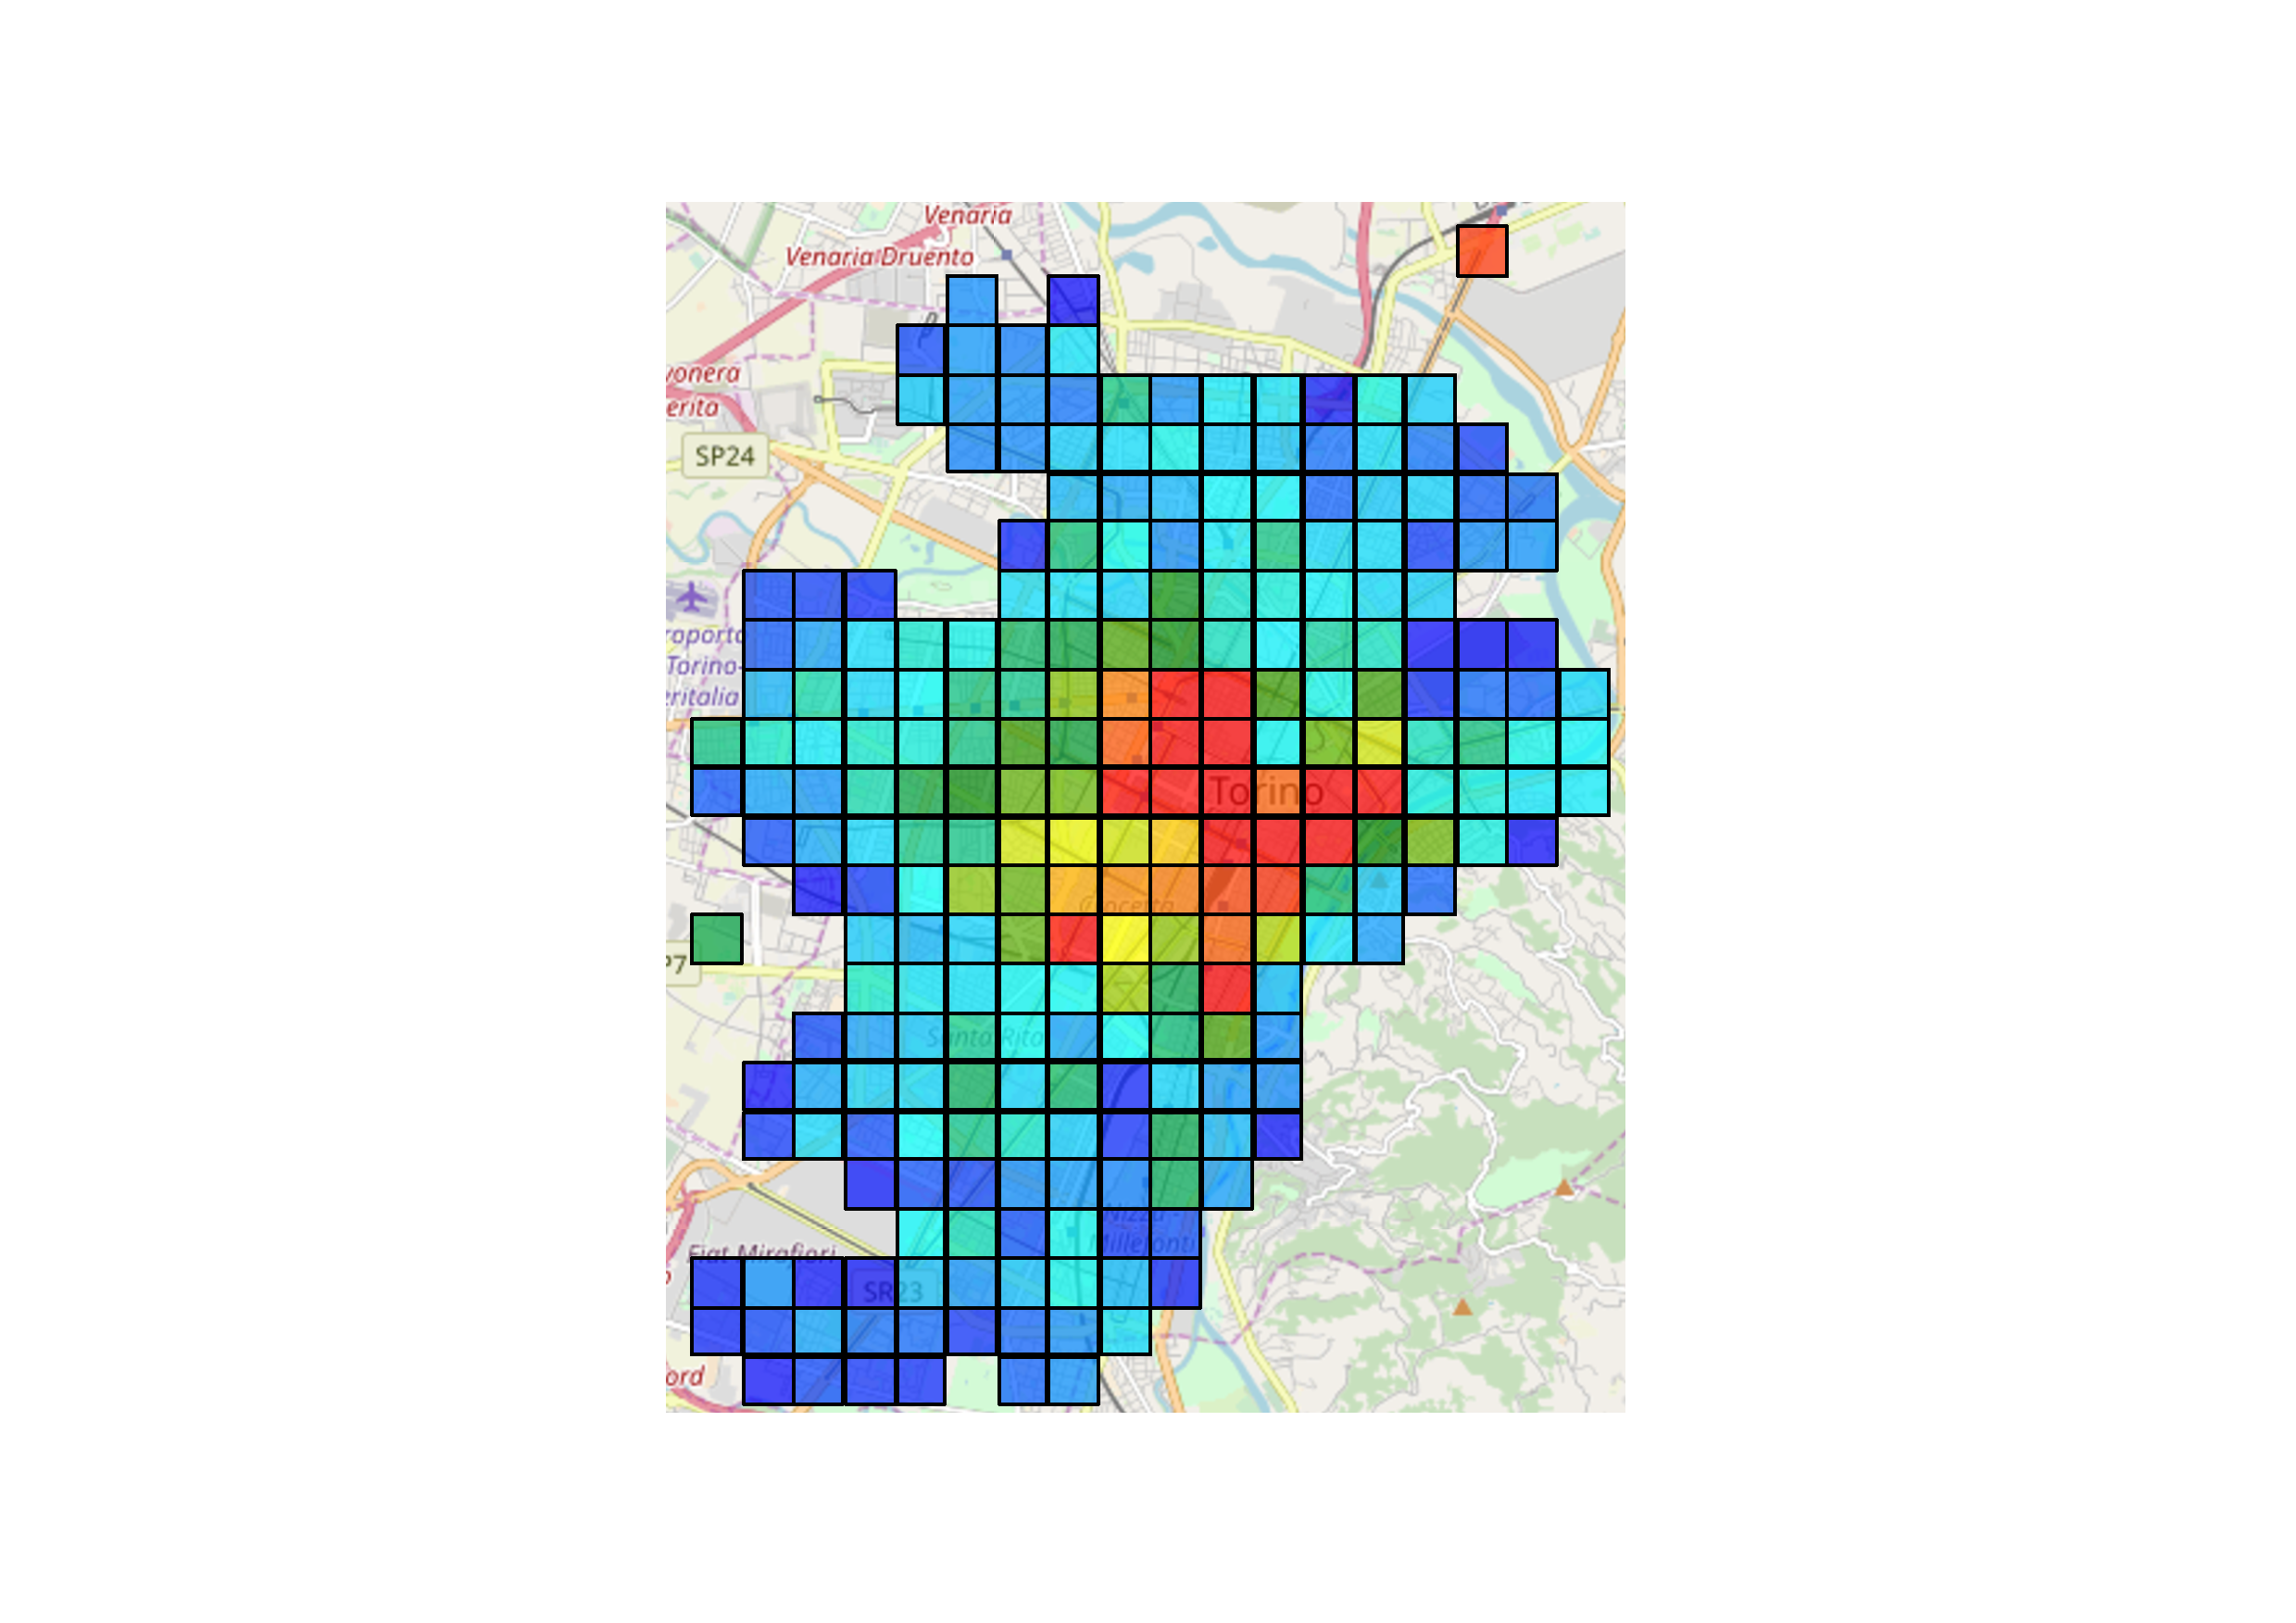
\includegraphics[width=0.35\columnwidth]{figures/Torino_NParkings.pdf}
%            }
%        \subfloat[][Average Parking Time.]
%            {
%            \label{fig:hm_avg-time}
%            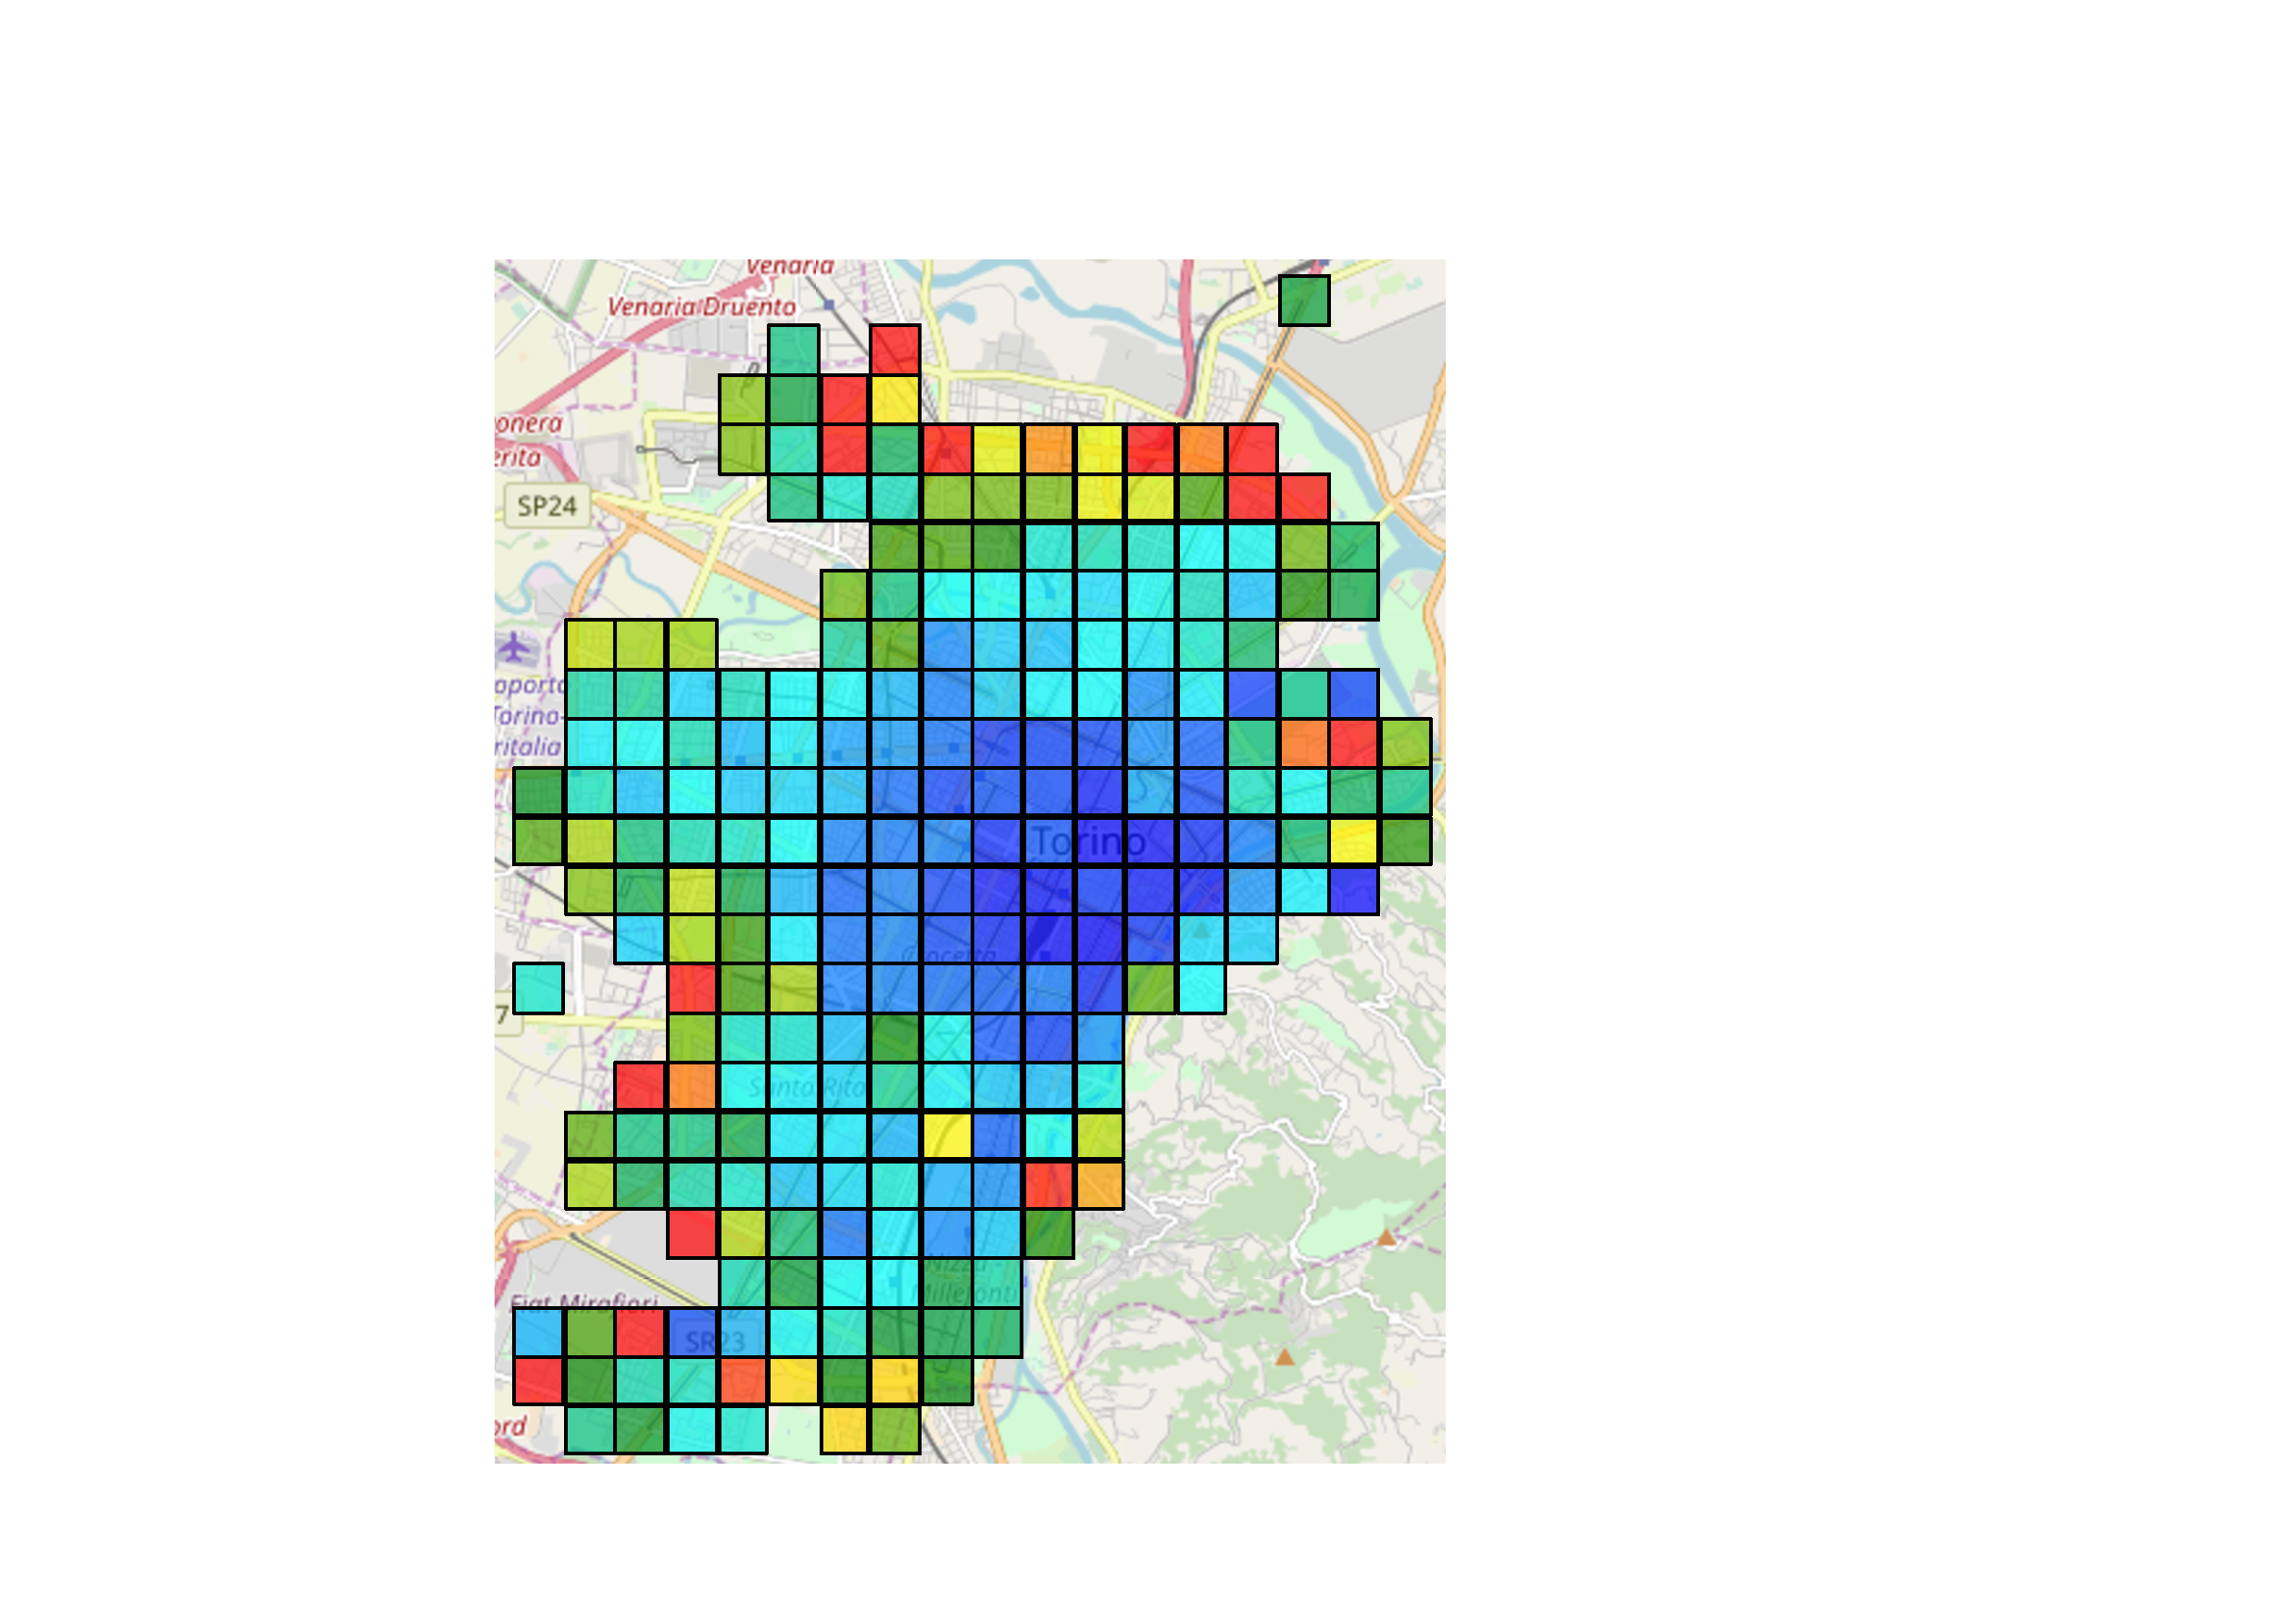
\includegraphics[width=0.35\columnwidth]{figures/Torino_AvgTime.pdf}
%            }
%    	\caption{Heatmaps showing (a) number of parkings per zone  and (b) average parking time per zone. Warmer areas have larger values. }
%    	\label{fig:data_car}
%\end{figure}

